% !TeX root = proposal.tex
\section{Proposed work --- vTask}
\label{sec:vTask}

The previous chapters in the proposed dissertation showed that
hypervisor-mediation API-remoting is the only effective mechanism for sharing
API-controlled compute devices among mutually distrustful tenants, e.g., in a
cloud computing environment. Virtualization vendors, such as VMware, have
begun adopting API-remoting based solutions for accelerator virtualization
\aak{cite BitFusion acquisition}.

API-remoting works by interposing on API calls invoked by the application in
the guest OS, and executing them in a surrogate, the API-server, in the host.
Typically, API-servers are associated with a single API framework (for
modularity and failure isolation between APIs/accelerators, and in order to be
able to use remote resources) and each API-server is a surrogate for a single
guest (to preserve memory isolation between guests). Applications that use
multiple accelerator API frameworks will be associated with multiple
API-servers, one per framework.

\begin{figure}[ht!]
\centering
\captionsetup{justification=centering,width=\linewidth}
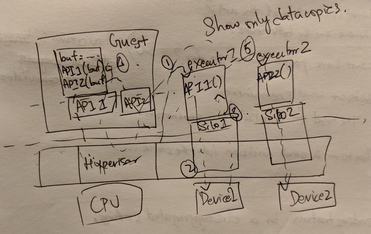
\includegraphics[width=0.5\linewidth]{figures/overview.png}
\caption{Data processed by two API stacks must pass through the guest application}
\label{fig:overview}
\end{figure}

Under a typical API-remoting system, applications that pipeline disparate accelerator frameworks are burdened with redundant data movement. All inter-accelerator data movement must take place in the guest application as that is where the accelerators are in the same logical address space. Figure~\ref{fig:overview} illustrates this scenario: when an \emph{API-1} function is invoked, associated data is copied from the \emph{guest application} to \emph{API-server-1}, and then to \emph{Device-1}’s memory. Once the function finishes executing on \emph{Device-1}, the result is copied back to the \emph{guest application}. When a function from \emph{API-2} is invoked, the same data (i.e., the output of the \emph{API-1 function}) is copied from the \emph{guest application} to \emph{API-server-2} and then to \emph{Device-2} to be processed.

In order to eliminate redundant data movement when an application uses multiple accelerators via API-remoting, the hypervisor must track the data passed to these API calls. The hypervisor must keep track of where the data flowed from and to, the validity of different copies of the data (e.g., if the data is modified on the accelerator, but hasn’t been copied back to the accelerator silo, or the guest application), and eliminate redundant data movement. As an example, if a guest application were to invoke the \texttt{cudaMempyDtoH()} function to copy data back from an Nvidia GPU, and then invoke the Intel QAT compression function \texttt{cpaDCCompressData2()} on the same data without modifying it in any way, the hypervisor should be able to detect this and elide the copying of data to and from the guest application. Further optimization may also be possible: peer-to-peer data copy between the devices if they are on the same machine, or by directly copying the data from the first API-server on one remote machine to the second API-server on another remote machine.

We propose to build vTask, an application-transparent data orchestration system that optimizes data movement among accelerators virtualized via API-remoting. vTask will leverage information from API annotations~\cite{ava-hotos} to track data buffers across the guest application, the API-servers servicing API calls made by the guest, and the accelerator hardware. vTask will optimize data movement across these components while ensuring that a coherent view of the data buffer is presented to anyone attempting to read the data. Ideally, vTask will require no changes to the guest application or  extra annotations of any kind from the application programmer. We hypothesize that annotations provided to virtualize the API (by the device or virtualization vendor) will be sufficient to infer the semantics of the data buffers managed.

We will prototype vTask in AvA, a state-of-the-art para-virtual API-remoting system for KVM. vTask will rely on device-side buffer allocation and deallocation API calls, and special annotations provided by LAPIS, AvA’s API description language, to determine buffer lifetime. Further, vTask will implement a simple MESI-style coherence protocol to track spatial validity of data (i.e., to track where the latest data is present). vTask will leverage optimizations such as shared memory, Unified Virtual Memory, and PCIe Peer-to-Peer (P2P) data transfer where available, but does not make assumptions about their universal availability.

vTask can handle data movement between both local and remote devices. When API-remoting to a remote system, the devices used by the guest application may be present on separate machines. We hypothesize that vTask will be able to eliminate costly data transfers over the network by adhering to the principle of lazy loading wherever possible, i.e., data is not moved until a demand fault occurs.

\aak{needed: a deeper explanation of design (breaking it down into the pieces that need to be built along with an estimation of how long each will take), a better evaluation strategy (with applications that we intend to run and how the machines will be setup, etc.)}